\documentclass{article} % say
\usepackage{tikz}
\usetikzlibrary{arrows,decorations.pathmorphing,backgrounds,positioning,fit,petri}
\begin{document}

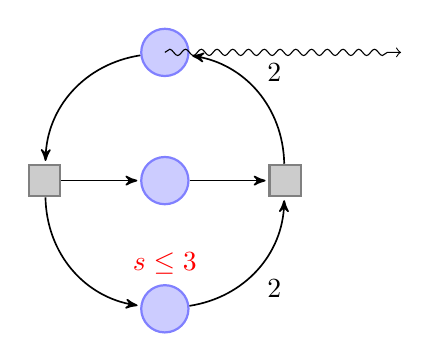
\begin{tikzpicture}
[place/.style={circle,draw=blue!50,fill=blue!20,thick,
inner sep=0pt,minimum size=6mm},
transition/.style={rectangle,draw=black!50,fill=black!20,thick,
inner sep=0pt,minimum size=4mm},every label/.style=red,
bend angle=40,
pre/.style={<-,shorten <=1pt,>=stealth',semithick},
post/.style={->,shorten >=1pt,>=stealth',semithick}]

\node[place] (waiting) {};
\node[place] (critical) [below=of waiting] {};

% We could use instead of 'above' or other position name, a number e.g. 60 for polar positioning
\node[place] (semaphore) [below=of critical, label=above:$s\le3$] {};
% \node[place] (semaphore) [below=of critical, label=60:$s\le3$] {};

\node[transition] (leave critical) [right=of critical] {}
	edge [pre] (critical)
	edge [post, bend right] node[auto,swap] {2} (waiting)
	edge [pre, bend left] node[auto] {2} (semaphore);
\node[transition] (enter critical) [left=of critical] {}
	edge [post] (critical)
	edge [pre,bend left] (waiting)
	edge [post,bend right] (semaphore);

% Without using edge styles:
%\node[transition] (enter critical) [left=of critical] {}
%	edge [->] (critical)
%	edge [<-,bend left=45] (waiting)
%	edge [->,bend right=45] (semaphore);

%% ----------- OTHER EDGE DRAWING OPTIONS    --------------%%
%% ----------- note: for this you must comment out --------------%%
%%------------ the last 4 lines starting with \node[transition].. --%%

% CONTROLS WITH ANCHORS: see pp 45-46 for node anchors and curve controls
% \node[transition] (enter critical) [left=of critical] {};
% \draw [->] (enter critical) -- (critical);
%\draw [->] (waiting) .. controls +(left:8mm) and +(up:8mm)
%.. (enter critical);

% USING to[out=<angle>,in=<angle>]:
% \node[transition] (enter critical) [left=of critical] {};
% \draw [->] (enter critical) -- (critical);
%\draw [->] (waiting) to [out=180,in=90] (enter critical);

% USING to [bend right=<angle>]:
% \node[transition] (enter critical) [left=of critical] {};
% \draw [->] (enter critical) -- (critical);
%\draw [->] (waiting) to [bend right=45] (enter critical);
%\draw [->] (enter critical) to [bend right=45] (semaphore);

% Or, instead of the semaphore label, we can use:
%  \node [red,above] at (semaphore.north) {$s\le 3$};


\draw [->,decorate,
decoration={snake,amplitude=.4mm,segment length=2mm,post length=1mm}]
(0,0) -- (3,0);


\end{tikzpicture}

\end{document}
